\documentclass[a4paper]{article}
\usepackage{amsfonts}
\usepackage{amsmath}
\usepackage{amssymb}
\usepackage{graphicx}  
\usepackage{cancel}

\newcommand{\degree}{^{\circ}}
\newcommand{\cis}{\operatorname{cis}}
\newcommand{\Bgsin}{\operatorname{Bgsin}}
\newcommand{\Bgcos}{\operatorname{Bgcos}}
\newcommand{\Bgtan}{\operatorname{Bgtan}}
\newcommand{\limit}{\lim\limits}
\newcommand{\summation}{\displaystyle\sum}
\newcommand{\dom}{\operatorname{dom}}

\begin{document}
  
\noindent \large Auteur: Rune Suy \\
\noindent \large Studierichting: Informatica\\
\noindent \large Oefeningenreeks 3H nr. 5.2\\

\medskip

\normalsize

$r=\sin\theta$\\

periode $= 2\pi$, beperk domein tot $[0,2\pi]$\\

$0=sin\theta \Leftrightarrow \theta \in \{0, \pi, 2\pi \}$\\

$r' = \cos\theta$\\

$0 = \cos\theta \Leftrightarrow \theta \in \left\{\dfrac{\pi}{2}, \dfrac{3\pi}{2}\right\}$\\

\begin{tabular}{c | c c c c c c c c c}
    $\theta$        & $0$ &     & $\dfrac{\pi}{2}$  &       & $\pi$ &       & $\dfrac{3\pi}{2}$ &     & $2\pi$\\\hline
    $r(\theta)$     & $0$ & $+$ & $+$               & $+$   & $0$   & $-$   & $-$               & $-$ & $0$\\
    $r'(\theta)$    & $+$ & $+$ & $0$               & $-$   & $-$   & $-$   & $0$               & $+$ & $+$\\\hline
    $r(\theta)$     & $\nearrow$ & $\nearrow$ & $M(1)$& $\searrow$& $\searrow$& $\searrow$& $m(-1)$& $\searrow$ & $\searrow$\\
\end{tabular}
\bigskip

Schets:\\

\begin{figure}[h]
    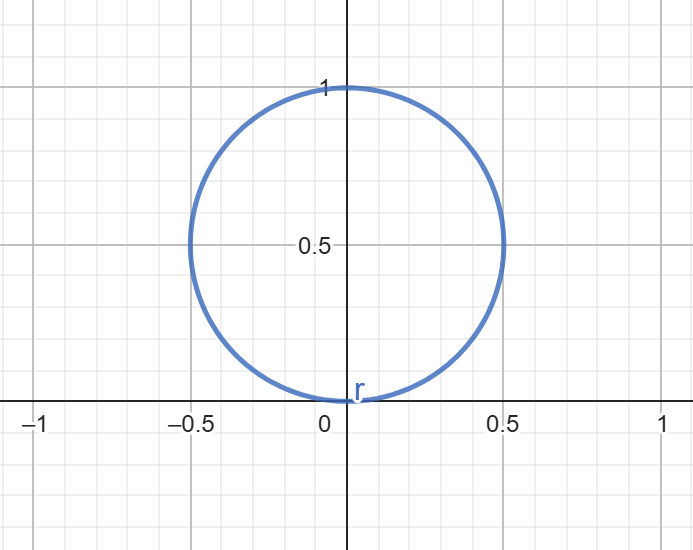
\includegraphics[width=\linewidth]{3H-5.2-rune.suy.INF.png}\\
\end{figure}

\begin{thebibliography}{999}
%\bibitem{a} Referentie
\end{thebibliography}
\end{document} 
